
To more concisely describe our approach, we write the DHT (\ref{eq:DHT}) as the
equivalent matrix-vector product with $\mtx{A} \in \R^{m \times n}$
\begin{equation}
    \vct{g} = \mtx{A}\vct{f}, \qquad \mtx{A}(j,k) = J_\nu(\omega_j r_k).
\end{equation}
The matrix $\mtx{A}$ is in general full rank and possesses complex oscillatory
structure. As a result, no straightforward fast algorithm exists to apply the
full matrix $\mtx{A}$ to a vector. However, we devise an NUFHT by noting that
certain \textit{blocks} $\mtx{A}(j_0:j_1, k_0:k_1)$ are able to be applied to a
vector rapidly using analytical expansions of the underlying Bessel function
$J_\nu$. 

\begin{figure}[!t]
  \centering
  \begin{subfigure}[b]{0.45\textwidth}
    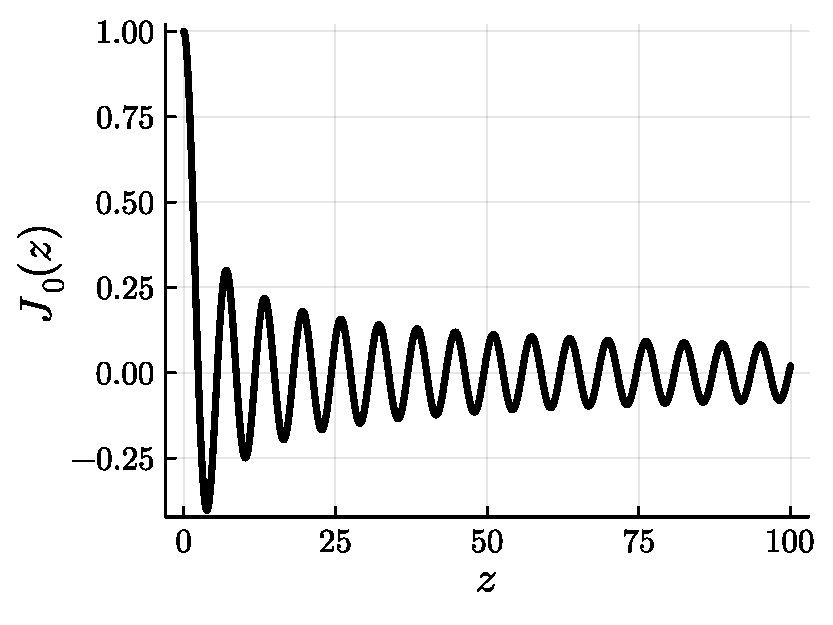
\includegraphics[width=\textwidth]{./figures/bessel_function.pdf}
  \end{subfigure}
  \begin{subfigure}[b]{0.45\textwidth}
    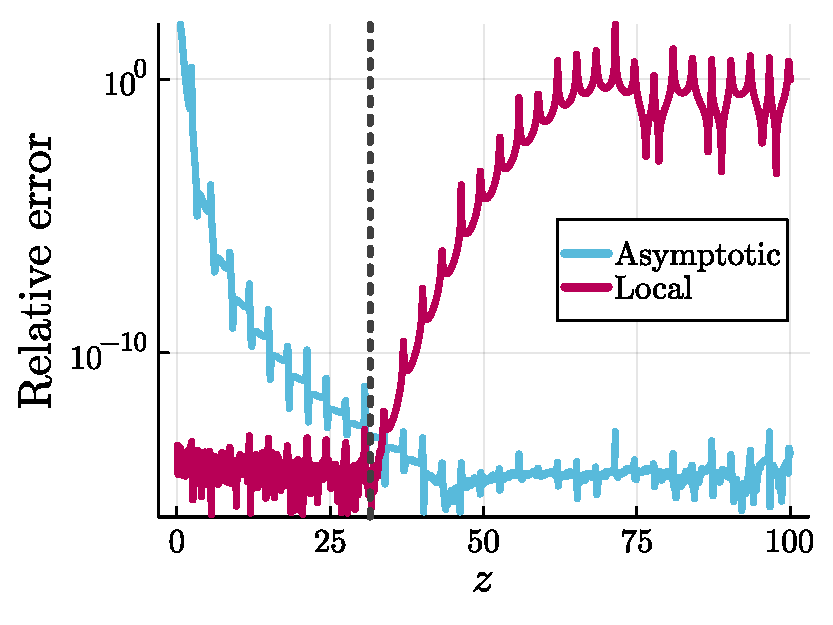
\includegraphics[width=\textwidth]{./figures/pointwise_errors.pdf}
  \end{subfigure}
  \caption{Bessel function $J_0(z)$ and pointwise relative error in
  approximating $J_0(z)$ using local and asymptotic expansions. Dotted vertical
  line shows crossover point where both expansions are accurate to $\epsilon =
  10^{-12}$.}
  \label{fig:two-expansions}
\end{figure}

When the argument $\omega_j r_k$ is small, $J_\nu$ is smooth and essentially
non-oscillatory, and we use a closed-form local expansion which approximates
$J_\nu$ in terms of Chebyshev polynomials, yielding a low-rank approximation to
the block $\mtx{A}(j_0:j_1, k_0:k_1)$ that can be applied to a vector in linear
time. When the argument $\omega_j r_k$ is large, we use a classical asymptotic
expansion which expresses $J_\nu$ as a sum of a small number of decaying
sinusoids, and can therefore be applied to a vector in quasilinear time using
the NUFFT. Figure~\ref{fig:two-expansions} shows the oscillatory behavior of
$J_0$, as well as the accuracy of these local and asymptotic expansions.

By analyzing the error in these two expansions, we can choose a threshold $z$
such that an $L$-term local expansion and an $M$-term asymptotic expansion are
both guaranteed to be accurate to the desired accuracy $\epsilon$ in the regions
$\omega_j r_k \leq z$ and $\omega_j r_k > z$ respectively. Next, we adaptively
subdivide $\mtx{A}$ into disjoint blocks so that either $\omega_j r_k \leq z$ or
$\omega_j r_k > z$ for all $\omega_j$ and all $r_k$ in each block. This leaves
only a few small blocks with $\omega_j r_k \approx z$ whose entries are directly
computed. Finally, we apply each of these disjoint blocks of $\mtx{A}$ to
$\vct{f}$ using the corresponding fast method. Figure~\ref{fig:subdivide} shows
an Hankel transform matrix $\mtx{A}$ divided into local and asymptotic entries
along the curve $\omega r = z$, as well as the corresponding adaptive
subdivision of the matrix into blocks which can be rapidly applied.

\begin{figure}
  \centering
  \newcommand\twa{0.29cm} \newcommand\tw{0.43cm}
  \begin{subfigure}[b]{0.28\textwidth}
    \begin{tikzpicture}
        \draw (0, 0) node[inner sep=0] {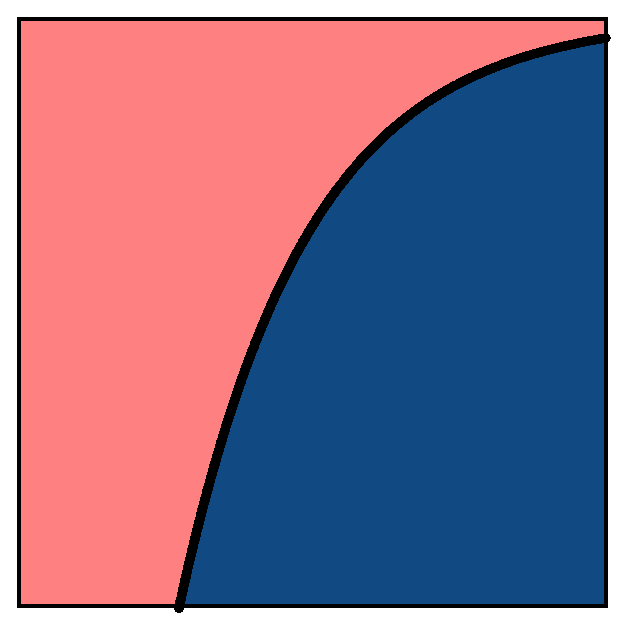
\includegraphics[width=0.75\textwidth,
        trim={\twa, \twa, \twa, \twa}, clip]{./figures/splitting.pdf}}; \draw
        (-0.8, 0.8) node {\small \textbf{Local}}; \draw (0.3, -0.7) node {\small
        \textbf{Asymptotic}}; \draw (0, 1.6) node {\small $r_1 \ \; < \ \dots \
        < \ \; r_n$}; \draw (-1.7, 0) node[align=center] {\small $\omega_1$
        \\[3pt] $\wedge$ \\[3pt] $\vdots$ \\[3pt] $\wedge$ \\[3pt] $\omega_m$};
    \end{tikzpicture}
    \caption{}
  \end{subfigure}
  \hspace*{0.0\textwidth}
  \begin{subfigure}[b]{0.21\textwidth}
    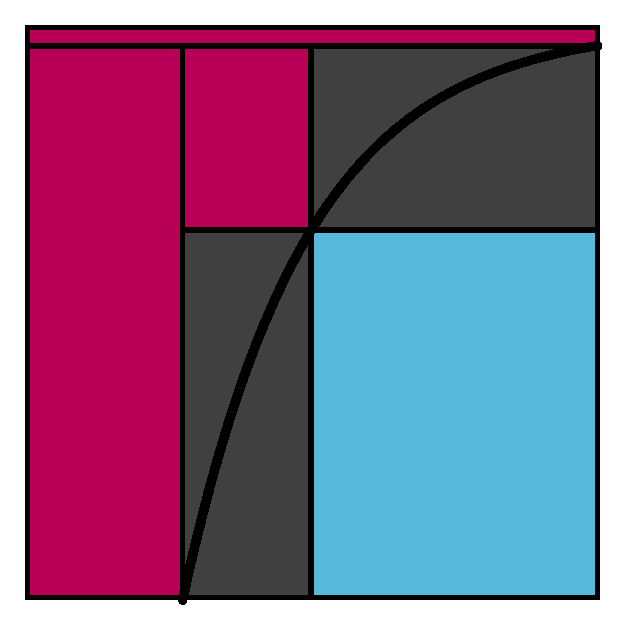
\includegraphics[width=\textwidth, trim={\tw, \tw, \tw, \tw}, clip]{./figures/splitting_lvl1.pdf}
    \caption{Level 1}
  \end{subfigure}
  \hfill
  \begin{subfigure}[b]{0.21\textwidth}
    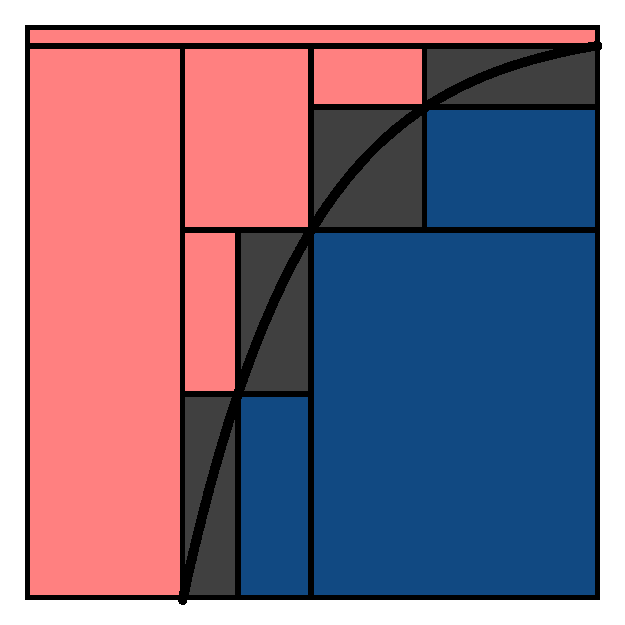
\includegraphics[width=\textwidth, trim={\tw, \tw, \tw, \tw}, clip]{./figures/splitting_lvl2.pdf}
    \caption{Level 2}
  \end{subfigure}
  \hfill
  \begin{subfigure}[b]{0.21\textwidth}
    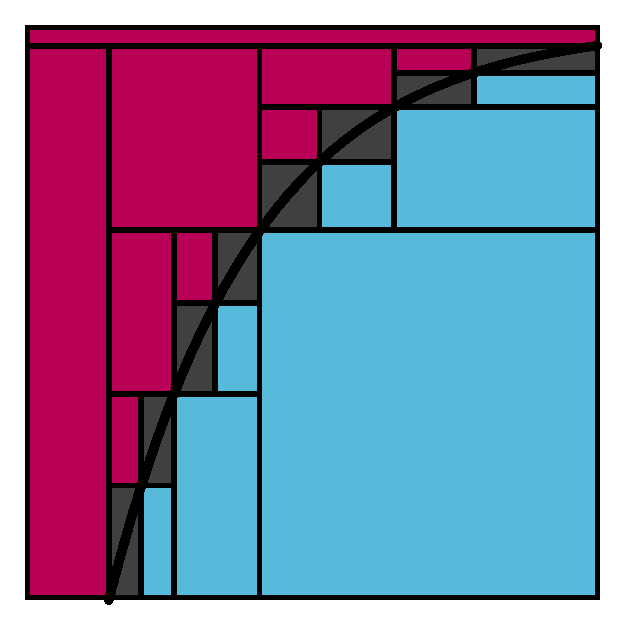
\includegraphics[width=\textwidth, trim={\tw, \tw, \tw, \tw}, clip]{./figures/splitting_lvl3.pdf}
    \caption{Level 3}
  \end{subfigure}
  \caption{Splitting of Hankel transform matrix $\mtx{A}$ along the curve
  $\omega r = z$ into local and asymptotic regions. Adaptive subdivision of
  $\mtx{A}$ into corresponding local (red), asymptotic (blue), and mixed (gray)
  sub-blocks at various levels.}
  \label{fig:subdivide}
\end{figure}